% Document Class ================================================================
\documentclass[final,5p,times]{elsarticle}
% Preamble ======================================================================
  %=================================== Equations ================================
  \usepackage{amsmath}            % maths
  %=================================== Images ===================================
  \usepackage{float}              % Make the images float
  \usepackage{subcaption}         % Sub-Plots
  \usepackage{transparent}
  %==================================== Tikz ====================================
  \usepackage{tikz}               % Construct tikz plots
    \usetikzlibrary{external}
    \tikzexternalize              %
  \usepackage{pgfplots}           % For tikz plots use pgf
  \pgfplotsset{compat=1.14}
  \usepgfplotslibrary{groupplots} % Use Libraries for group pgf
  %\usetikzlibrary{calc}
  %\usetikzlibrary{shapes.geometric, arrows, mindmap, external} % Diagrams in Tikz

% !TEX program = shell-escape
% Definition ====================================================================
\newlength\figureheight
\newlength\figurewidth
\setlength\figurewidth{8.3cm}
\setlength\figureheight{6cm}
\newcommand{\includetikz}[1]{%
  \tikzsetnextfilename{#1}%
  \input{#1.tex}%
}

\begin{document} 
  %\pgfplotsset{compat=newest}
  \pgfplotsset{compat=1.11}
  \begin{figure}[H]   % Figure 1
    \centering
    %\includegraphics[keepaspectratio,width=5cm]{images/1654542416421.pdf}
    %% Creator: Inkscape inkscape 0.92.5, www.inkscape.org
%% PDF/EPS/PS + LaTeX output extension by Johan Engelen, 2010
%% Accompanies image file 'layout_vib.pdf' (pdf, eps, ps)
%%
%% To include the image in your LaTeX document, write
%%   \input{<filename>.pdf_tex}
%%  instead of
%%   \includegraphics{<filename>.pdf}
%% To scale the image, write
%%   \def\svgwidth{<desired width>}
%%   \input{<filename>.pdf_tex}
%%  instead of
%%   \includegraphics[width=<desired width>]{<filename>.pdf}
%%
%% Images with a different path to the parent latex file can
%% be accessed with the `import' package (which may need to be
%% installed) using
%%   \usepackage{import}
%% in the preamble, and then including the image with
%%   \import{<path to file>}{<filename>.pdf_tex}
%% Alternatively, one can specify
%%   \graphicspath{{<path to file>/}}
%% 
%% For more information, please see info/svg-inkscape on CTAN:
%%   http://tug.ctan.org/tex-archive/info/svg-inkscape
%%
\begingroup%
  \makeatletter%
  \providecommand\color[2][]{%
    \errmessage{(Inkscape) Color is used for the text in Inkscape, but the package 'color.sty' is not loaded}%
    \renewcommand\color[2][]{}%
  }%
  \providecommand\transparent[1]{%
    \errmessage{(Inkscape) Transparency is used (non-zero) for the text in Inkscape, but the package 'transparent.sty' is not loaded}%
    \renewcommand\transparent[1]{}%
  }%
  \providecommand\rotatebox[2]{#2}%
  \newcommand*\fsize{\dimexpr\f@size pt\relax}%
  \newcommand*\lineheight[1]{\fontsize{\fsize}{#1\fsize}\selectfont}%
  \ifx\svgwidth\undefined%
    \setlength{\unitlength}{5cm}%
    \ifx\svgscale\undefined%
      \relax%
    \else%
      \setlength{\unitlength}{\unitlength * \real{\svgscale}}%
    \fi%
  \else%
    \setlength{\unitlength}{\svgwidth}%
  \fi%
  \global\let\svgwidth\undefined%
  \global\let\svgscale\undefined%
  \makeatother%
  \begin{picture}(1,1.76456311)%
    \lineheight{1}%
    \setlength\tabcolsep{0pt}%
    \put(0,0){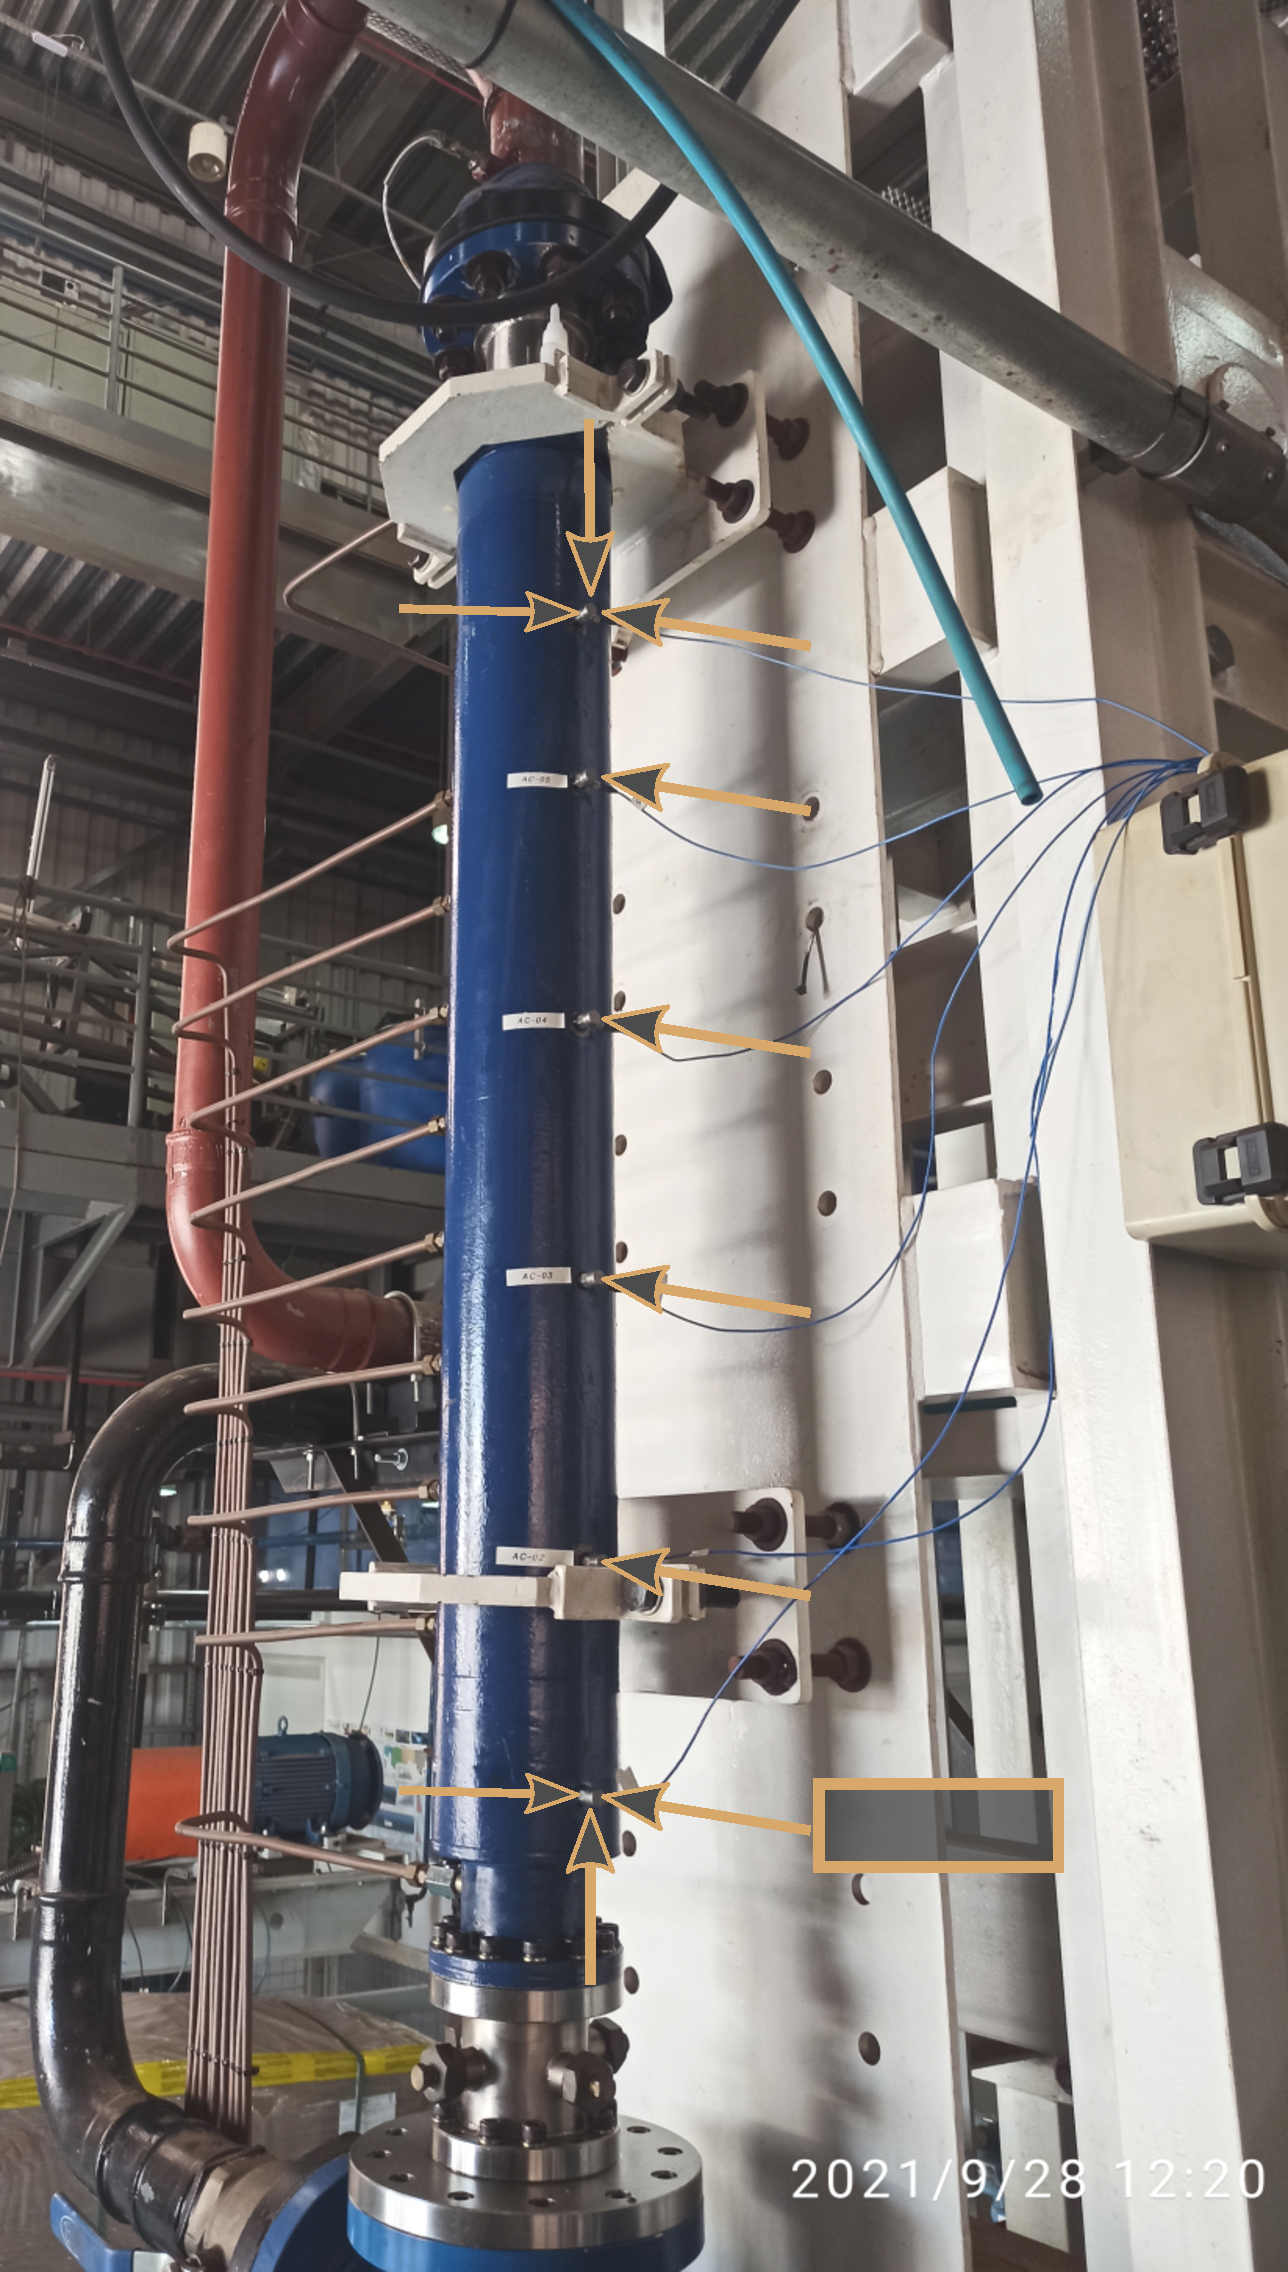
\includegraphics[width=\unitlength,page=1]{layout_vib.pdf}}%
    \put(0.745,0.24265345){\color[rgb]{0.84705882,0.65882353,0.41960784}\transparent{0.98000002}\makebox(0,0)[lt]{\lineheight{1.25}\smash{\begin{tabular}[t]{l} \tiny AC-01X\end{tabular}}}}%
    \put(0,0){\includegraphics[width=\unitlength,page=2]{layout_vib.pdf}}%
    \put(0.755,0.44639141){\color[rgb]{0.84705882,0.65882353,0.41960784}\transparent{0.98000002}\makebox(0,0)[lt]{\lineheight{1.25}\smash{\begin{tabular}[t]{l} \tiny AC-02\end{tabular}}}}%
    \put(0,0){\includegraphics[width=\unitlength,page=3]{layout_vib.pdf}}%
    \put(0.755,0.69157861){\color[rgb]{0.84705882,0.65882353,0.41960784}\transparent{0.98000002}\makebox(0,0)[lt]{\lineheight{1.25}\smash{\begin{tabular}[t]{l} \tiny AC-03\end{tabular}}}}%
    \put(0,0){\includegraphics[width=\unitlength,page=4]{layout_vib.pdf}}%
    \put(0.755,0.90505636){\color[rgb]{0.84705882,0.65882353,0.41960784}\transparent{0.98000002}\makebox(0,0)[lt]{\lineheight{1.25}\smash{\begin{tabular}[t]{l} \tiny AC-04\end{tabular}}}}%
    \put(0,0){\includegraphics[width=\unitlength,page=5]{layout_vib.pdf}}%
    \put(0.755,1.11443992){\color[rgb]{0.84705882,0.65882353,0.41960784}\transparent{0.98000002}\makebox(0,0)[lt]{\lineheight{1.25}\smash{\begin{tabular}[t]{l} \tiny AC-05\end{tabular}}}}%
    \put(0,0){\includegraphics[width=\unitlength,page=6]{layout_vib.pdf}}%
    \put(0.745,1.29249431){\color[rgb]{0.84705882,0.65882353,0.41960784}\transparent{0.98000002}\makebox(0,0)[lt]{\lineheight{1.25}\smash{\begin{tabular}[t]{l} \tiny AC-06X\end{tabular}}}}%
    \put(0,0){\includegraphics[width=\unitlength,page=7]{layout_vib.pdf}}%
    \put(0.19550434,0.33449444){\color[rgb]{0.84705882,0.65882353,0.41960784}\transparent{0.98000002}\makebox(0,0)[lt]{\lineheight{1.25}\smash{\begin{tabular}[t]{l} \tiny AC-01Y\end{tabular}}}}%
    \put(0,0){\includegraphics[width=\unitlength,page=8]{layout_vib.pdf}}%
    \put(0.57315522,0.13519379){\color[rgb]{0.84705882,0.65882353,0.41960784}\transparent{0.98000002}\makebox(0,0)[lt]{\lineheight{1.25}\smash{\begin{tabular}[t]{l} \tiny AC-01Z\end{tabular}}}}%
    \put(0,0){\includegraphics[width=\unitlength,page=9]{layout_vib.pdf}}%
    \put(0.57315522,1.41753084){\color[rgb]{0.84705882,0.65882353,0.41960784}\transparent{0.98000002}\makebox(0,0)[lt]{\lineheight{1.25}\smash{\begin{tabular}[t]{l} \tiny AC-06Z\end{tabular}}}}%
    \put(0,0){\includegraphics[width=\unitlength,page=10]{layout_vib.pdf}}%
    \put(0.19550434,1.22549675){\color[rgb]{0.84705882,0.65882353,0.41960784}\transparent{0.98000002}\makebox(0,0)[lt]{\lineheight{1.25}\smash{\begin{tabular}[t]{l} \tiny AC-06Y\end{tabular}}}}%
    \put(0,0){\includegraphics[width=\unitlength,page=11]{layout_vib.pdf}}%
    \put(0.28 ,0.175){\color[rgb]{1,1,1}\makebox(0,0)[lt]{\lineheight{1.25}\smash{\begin{tabular}[t]{l} \tiny {$P_1$}\end{tabular}}}}%
    \put(0,0){\includegraphics[width=\unitlength,page=12]{layout_vib.pdf}}%
    \put(0.28 ,1.140){\color[rgb]{1,1,1}\makebox(0,0)[lt]{\lineheight{1.25}\smash{\begin{tabular}[t]{l} \tiny {$P_9$}\end{tabular}}}}%
    \put(0,0){\includegraphics[width=\unitlength,page=13]{layout_vib.pdf}}%
    \put(0.568,0.052){\color[rgb]{1,1,1}\makebox(0,0)[lt]{\lineheight{1.25}\smash{\begin{tabular}[t]{l} \tiny {$T_2$}\end{tabular}}}}%
    \put(0,0){\includegraphics[width=\unitlength,page=14]{layout_vib.pdf}}%
    \put(0.512,1.682){\color[rgb]{1,1,1}\makebox(0,0)[lt]{\lineheight{1.25}\smash{\begin{tabular}[t]{l} \tiny {$T_3$}\end{tabular}}}}%
  \end{picture}%
\endgroup%

    \caption{Sensors Distribution.}
    \label{fig.2}
  \end{figure}
  % =============================================================================
  \begin{figure}[H]         %Figure 1
    \centering
    \includetikz{H}
  \end{figure}
  % =============================================================================
  \begin{figure}[H]         %Figure 2
    \centering
    \includetikz{Ta}
  \end{figure}
  % =============================================================================
  \begin{figure}[H]         %Figure 2
    \centering
    \includetikz{mu}
  \end{figure}
  % =============================================================================
  \begin{figure}[H]         %Figure 3
    \centering
    \includetikz{sigmoid}
    \caption{40 [Hz], 169 [mPa-s], 28 [\(\displaystyle \mathrm{m^3/h}\)]}
  \end{figure}
  % =============================================================================
  \begin{figure*}[!ht]      %Figure 4.1
    \centering
    \begin{tabular}{l}
      \begin{subfigure}{7.8cm}
        \includetikz{AC-02}
      \end{subfigure}
      ~\hspace{-20mm}~
      \begin{subfigure}{8.3cm}
        \includetikz{AC-03}
      \end{subfigure}
      \\
      ~\vspace{-7mm}~
      \\
      \begin{subfigure}{7.8cm}
        \includetikz{AC-04}
      \end{subfigure}
      ~\hspace{-20mm}~
      \begin{subfigure}{8.3cm}
        \includetikz{AC-05}
      \end{subfigure}
    \end{tabular}
  \end{figure*}
  % =============================================================================
  %\begin{figure*}[!ht]      %Figure 4.2
    %\centering
    %\begin{tabular}{l}
    %  \begin{subfigure}{5.9cm}
    %    \includetikz{AC-01X}
    %  \end{subfigure}
    %  ~\hspace{-8mm}~
    %  \begin{subfigure}{4.8cm}
    %  \end{subfigure}
    %  ~\hspace{-8mm}~
    %  \begin{subfigure}{6.2cm}
    %    \includetikz{AC-01Z}
    %  \end{subfigure}
    %  \\
    %  ~\vspace{-6mm}~
    %  \\
    %  \begin{subfigure}{5.9cm}
    %    \includetikz{AC-06X}
    %  \end{subfigure}
    %  ~\hspace{-8mm}~
    %  \begin{subfigure}{4.8cm}
    %    \includetikz{AC-06Y}
    %  \end{subfigure}
    %  ~\hspace{-8mm}~
    %  \begin{subfigure}{6.2cm}
    %    \includetikz{AC-06Z}
    %  \end{subfigure}
    %  \\
    %\end{tabular}
  %\end{figure*}
  % =============================================================================
  \begin{figure}[H]         %Figure 5
    \centering
    \includetikz{fft_AC-04_0-750Hz}
    \caption{AC-04 0-750 Hz}
  \end{figure}
  % =============================================================================
  \begin{figure}[H]         %Figure 6
    \centering
    \includetikz{fft_AC-01Z_1-5kHz}
    \caption{AC-01Z 1-5kHz}
  \end{figure}
  % =============================================================================
  \clearpage
  \begin{figure}[H]         %Figure 7
    \centering
    \includetikz{ranges_AC-04_6_kHz}
    \includetikz{ranges_AC-04_1_kHz}
    \caption{Analysis ranges AC-04 sensor at 72.9\% water cut}
  \end{figure}
  % =============================================================================
  \begin{figure}[H]         %Figure 8
    \centering
    \includetikz{pearson1}
    \caption{Pearson correlation with the dimensionless torque}
    \label{fig.8} 
  \end{figure}
  \begin{figure}[H]         %Figure 8.1
    \centering
    \includetikz{pearson2}
    \caption{Dimensionless torque vs rms of fft between 0 - 250 Hz for AC-01Y sensor}
    \label{fig.8.1} 
  \end{figure}
  % =============================================================================
  \begin{figure*}[!ht]      %Figure 8
    \centering
    \includetikz{fft_rms_0-250Hz_AC-01Y}
  \end{figure*}
  % =============================================================================
  \begin{figure*}[!ht]      %Figure 9
    \centering
    \includetikz{fft_rms_0-250Hz_AC-06Z}
  \end{figure*}
  % =============================================================================
  \begin{figure}[H]         %Figure 10
    \centering
    \includetikz{logit_fft_rms_0-250Hz_AC-01Y}
    \caption{AC-01Y}
  \end{figure}
  % =============================================================================
  \begin{figure}[H]         %Figure 11
    \centering
    \includetikz{logit_fft_rms_0-250Hz_AC-04}
    \caption{AC-04}
  \end{figure}
  %% =============================================================================
  \begin{figure}[H]         %Figure 12
    \centering
    \includetikz{logit_fft_rms_0-250Hz_AC-06Y}
    \caption{AC-06Y}
  \end{figure}
  % =============================================================================
  \begin{figure}[H]         %Figure 14
    \centering
    \includetikz{comparisson}
  \end{figure}
  % =============================================================================
  %\begin{figure}[H]         %Figure 15
  %  \centering
  %  \setlength\figurewidth{7cm}
  %  \setlength\figureheight{7cm}
  %  \setlength\figurewidth{\figurewidth}
  %  \includetikz{bound_train}
  %\end{figure}
  % =============================================================================
  %\begin{figure}[H]         %Figure 16
  %  \centering
  %  \setlength\figurewidth{7cm}
  %  \setlength\figureheight{7cm}
  %  \setlength\figurewidth{\figurewidth}
  %  \includetikz{bound_test}
  %\end{figure}

\end{document}